\section{Proposed Method}

As previously mentioned we start with a set of specifications for a \gls{MVP}. From there, we will then add features according to a ranked feature list. See specifications in the subsections below.

\subsection{Sensor setup}\label{sec:sensor-setup}
The sensors that the XC90 are equipped with are:
\begin{itemize}
\item Stereo Cameras (Autoliv)
\item GPS+IMU (Applanix LV V5,
  \url{https://www.applanix.com/downloads/products/specs/POSLV_DS_feb_2017_yw.PD
  })
\item  \gls{LIDAR} (Velodyne HD132E)
\item  Radars
\item  Radio based localization (5G).
\item  Wheel encoders
\end{itemize}

Since the idea is that the data will be “crowd sourced” the sensors
need to be fairly cheap so that they likely are equipped on many
cars. We will therefore not consider \gls{LIDAR}. We will, however, look
into radio based localization using the 5G standard, this is not yet
present in any cars, but may be in the near future.

\subsection{\gls{MVP}}

The \gls{MVP} is the general problem scaled down and simplifying
assumptions made, while still considered to be a relevant problem. We make the following
simplification/assumptions:
\begin{itemize}
\item Evaluation of one data-set
\item Static environment
\item Assume all the sensors are calibrated
\item ``Small dataset'', being able to compute on personal computer
\end{itemize}
This scenario could correspond to:
\begin{enumerate}
\item Drive to work and record a single sensor data-set
\item Perform offline computation
\item Drive the same road to work and navigate using the map
\end{enumerate}
The minimum set of sensors to consider are:
\begin{itemize}
\item GPS
\item Stereo Cameras
\item IMU
\item Radio receivers
\end{itemize}

The localization part should be able to handle multiple sensor types as well as different combinations of them to increase robustness.


The system will be evaluated using datasets from
\url{http://robotcar-dataset.robots.ox.ac.uk/}

\subsection{Minimum viable solution}


The \gls{MVS} solves the \gls{MVP}, and thus only implements the necessary
features.
\begin{itemize}
\item A sensor fusion algorithm is used to combine the information
  from different sensors including camera, LIDAR, USRP, channel
  sounder.
\item Estimate and track the position of the vehicle based on a SLAM
  algorithm.
\end{itemize}

The trajectory of the car over T time steps can be described as   and
the positions of the landmarks can be described as, which can be
considered to be static in time. Then the \gls{SLAM} problem solves
the following filtering problem.

To include radio measurements there are two options:
\begin{itemize}
\item To use a USRP with LTE framework and switching antenna array to
  receive commercial LTE signals from base stations, estimate the
  Angle of Arrival, and time delay of multipath components.
\item To use channel sounder and antenna arrays (with 32 antenna
  elements) on both base station and user sides to collect channel
  information with respect to angles and distances.
\end{itemize}

\subsection{Features include after MVP (ranked)}

Listed below are features are considered ``good to have'' but not
necessary:

\begin{itemize}
\item Radio localization  (Xuhong  Junshi)
\item Updating map:
  \begin{itemize}
  \item Update the map dynamically over time.
  \item Multiple data-sets from the same area.
  \end{itemize}
\item Large scale mapping (country size)
\item How to extract persistent features in the environment, that does
  not change over time:
  \begin{itemize}
  \item  Semantic segmentation (labelling of objects, not only ORB
    features), lanes will give lateral information, emergency doors
    will give information in the tunnel, stop signs will give
    longitudinal location
  \end{itemize}
\item Feature extractor for lanes.
\item Feature extractor for signs.
\item Handle sensor failures.
\item Include calibration parameters of the sensors in the offline processing.
\item Be able to handle different types of sensors, such as different camera types, e.g. normal lens, fish lens, HD camera.
\end{itemize}

\subsection{Feature extraction camera}

The landmarks extracted from the camera can be done using semantic
segmentation on the data-set \cite{Brostow:2009:SOC:1464534.1465403}.

Tutorial is found here:
\url{https://se.mathworks.com/help/vision/examples/semantic-segmentation-using-deep-learning.html}

From the segmented images, it is possible to get an \gls{AOA}
measurement. From the image, the center of gravity can be computed,
and can be compared with the field of view of the sensing camera.

\subsection{Motion model}
As a motion model for sensor fusion we will use the bicycle model adapted for a car.
The parameters are shown in figure \ref{fig:motion_model}. The state space model is defined as

\begin{equation}
 \begin{array}[b]{r}
  \dot{x} = v \cos \theta \\
  \dot{y} = v \sin \theta \\
  \dot{\theta} = \frac{v}{L} \tan{\phi}
 \end{array}
\end{equation}

where $v$ is speed of the car and $\phi$ is the steering angle. 
These can be observed using an IMU and/or estimates from the onboard car sensors.


\begin{figure}
\label{fig:motion_model}
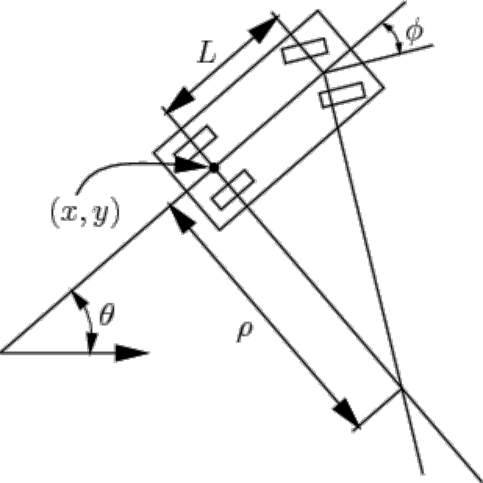
\includegraphics[width=0.3\textwidth]{figures/bicycle_model.pdf}
\caption{Bicycle motion model adapted for car}
\end{figure}



\subsection{Performance assessment}

In order to assess the performance of the offline \gls{SLAM}
algorithm, it is possible to perform cross-validation.

\subsection{Research arenas (WARA-CAT)}


The requirements on WARA-CAT are:
\begin{itemize}
\item A vehicle (with similar size of Volvo V70) or a manually moved
  trolley to accommodate the sensors.
\item Radio equipment :
  \begin{itemize}
  \item   antenna arrays,
  \item  channel sounder,
  \item USRP,
  \item laptop
  \end{itemize}
  \item Test environment for data collection using the defined sensor in
    \ref{sec:sensor-setup}
\item 5G network for radio localization.
\item Ground truth of the vehicle for evaluation of algorithms.
\end{itemize}


%%% Local Variables:
%%% mode: latex
%%% TeX-master: "main"
%%% End:
